
\documentclass[a4paper,12pt]{article}
\usepackage{enumitem} % -> Alphabetical Lists
\usepackage{amsmath} % -> Matrices
\usepackage{fullpage} % -> A4 Full Page
\usepackage{amssymb} % -> Therefore
\usepackage[utf8]{inputenc}
\usepackage{graphicx}
\usepackage{adjustbox}
\usepackage{listings}
\usepackage{braket}
\usepackage{geometry}
\usepackage{tikz}
\usepackage{graphicx}
\usepackage{commath}
\usetikzlibrary{quantikz}

\graphicspath{ {./} }

\geometry{
    a4paper,
    total={220mm,257mm},
    left=0mm,
    top=20mm,
}

\title{Quantum Computing Assignment 4 - Group 18}
\author{
    Rallabhandi, Anand Krishna 
    \and
    Mustafa, Syed Husain
    \and
     , Mohammed Kamran 
}
\date{\today}

\begin{document}

\maketitle

\section*{Exercise 5.1 \\Bell Inequality}

 (Bell states and superdense coding)

\begin{enumerate}[label=(\alph*)]
    \item\phantom{-} \\
        Given : $\ket{0} = \alpha\ket{a}+ \beta\ket{b}\hspace{1mm}\&\hspace{1mm}\ket{1}=\gamma\ket{a}+\delta\ket{b}$, where $\{\ket{a},\ket{b}\}$ is the orthonormal basis of $\mathbb{C}^{2}$\\~\\
        Consider $\frac{1}{\sqrt{2}}(\ket{01}-\ket{10})$ \\
        $\ket{01}=\ket{0} \otimes \ket{1} \implies \ket{01} = \begin{pmatrix}
            \alpha a\begin{pmatrix}
                \gamma a \\
                \delta b \\
            \end{pmatrix} \\
            \beta b\begin{pmatrix}
                \gamma a \\
                \delta b \\
            \end{pmatrix}  
        \end{pmatrix}
        \implies \ket{01} =\Big( \alpha\gamma\ket{aa} + \alpha\delta\ket{ab} + \beta\gamma\ket{ba} + \beta\delta\ket{bb}\Big) \hspace{5mm} \textbf{(I)}$ \\~\\
        $\ket{10}=\ket{1} \otimes \ket{0} \implies \ket{10} = \begin{pmatrix}
            \gamma a\begin{pmatrix}
                \alpha a \\
                \beta b \\
            \end{pmatrix} \\
            \delta b\begin{pmatrix}
                \alpha a \\
                \beta b \\
            \end{pmatrix}  
        \end{pmatrix}
        \implies \ket{10} =\Big( \alpha\gamma\ket{aa} + \beta\gamma\ket{ab} + \alpha\delta\ket{ba} + \beta\delta\ket{bb}\Big) \hspace{5mm} \textbf{(II)}\\~\\$
        $\frac{1}{\sqrt{2}}\Big(\textbf{(I)}-\textbf{(II)}\Big) = \frac{1}{\sqrt{2}}\begin{pmatrix}
            \alpha\gamma aa - \alpha\gamma aa \\
            \alpha\delta ab - \beta\gamma \\
            \beta\gamma ba - \alpha\delta ba\\
            \beta\delta bb - \beta\delta bb\\
        \end{pmatrix} = \frac{1}{\sqrt{2}}(\alpha\delta - \beta\gamma)\frac{\ket{ab}-\ket{ba}}{\sqrt{2}}$
        \[\therefore \frac{\ket{01}\ket{10}}{\sqrt{2}} = (\alpha\delta - \beta\gamma)\frac{\ket{ab}-\ket{ba}}{\sqrt{2}}\]\\~\\
    \item\phantom{-} \\
        Given, $\ket{\psi} = \frac{1}{\sqrt{2}}\big(\ket{01}-\ket{10}\big)\equiv \frac{1}{\sqrt{2}}\begin{pmatrix}
            \phantom{-}0\phantom{-} \\
            \phantom{-}1\phantom{-} \\
            -1\phantom{-} \\
            \phantom{-}0\phantom{-}
        \end{pmatrix} = \ket{\beta_{11}}$\\
        $Q=Z=\begin{pmatrix}
            1 & \phantom{-}0 \\
            0 & -1 \\
        \end{pmatrix},\hspace{2mm}R=X=\begin{pmatrix}
            0 & 1 \\
            1 & 0 \\
        \end{pmatrix}$ \\
        $S = \frac{1}{\sqrt{2}}(-Z-X)=\frac{1}{\sqrt{2}}\begin{pmatrix}
            -\begin{pmatrix}
               1 & \phantom{-}0\\ 
               0 & -1\\
            \end{pmatrix} - \begin{pmatrix}
                0 & 1 \\
                1 & 0 \\
            \end{pmatrix}
        \end{pmatrix} = \frac{1}{\sqrt{2}}\begin{pmatrix}
            -1 & -1 \\
            -1 & \phantom{-}1 \\
        \end{pmatrix}$ \\
        $T = \frac{1}{\sqrt{2}}(Z-X)=\frac{1}{\sqrt{2}}\begin{pmatrix}
            \begin{pmatrix}
               1 & \phantom{-}0\\ 
               0 & -1\\
            \end{pmatrix} - \begin{pmatrix}
                0 & 1 \\
                1 & 0 \\
            \end{pmatrix}
        \end{pmatrix} = \frac{1}{\sqrt{2}}\begin{pmatrix}
            \phantom{-}1 & -1 \\
            -1 & -1 \\
        \end{pmatrix}$ \\
        \begin{enumerate}[label=(\roman*)]

            \item $\bra{\psi}Q\otimes S\ket{\psi} = \frac{1}{2\sqrt{2}}\begin{pmatrix}
                0 & 1 & -1 & 0
            \end{pmatrix} \begin{pmatrix}
                -1 & -1 & \phantom{-}0 & \phantom{-}0\\
                -1 & \phantom{-}1 & \phantom{-}0 &\phantom{-}0 \\
                \phantom{-}0 & \phantom{-}0 & \phantom{-}1 & \phantom{-}1 \\
                \phantom{-}0 & \phantom{-}0 & \phantom{-}1 & -1 \\
            \end{pmatrix}\begin{pmatrix}
                \phantom{-}0 \\
                \phantom{-}1 \\
                -1\\
                \phantom{-}0\\
            \end{pmatrix}=\frac{1}{2\sqrt{2}}\begin{pmatrix}
                -1 & 1 & -1 & -1\\
            \end{pmatrix} \begin{pmatrix}
                \phantom{-}0 \\
                \phantom{-}1 \\
                -1 \\
                \phantom{-}0 \\
            \end{pmatrix} = \frac{1}{\sqrt{2}}$

            \item $\bra{\psi}R\otimes S\ket{\psi} = \frac{1}{2\sqrt{2}}\begin{pmatrix}
                0 & 1 &-1 &0
            \end{pmatrix}\begin{pmatrix}
                \phantom{-}0 & \phantom{-}0 & -1 & -1 \\
                \phantom{-}0 & \phantom{-}0 & -1 & \phantom{-}1 \\
                -1 & -1 &\phantom{-}0 & \phantom{-}0\\
                -1 & \phantom{-}0 & \phantom{-}0 & \phantom{-}0\\
            \end{pmatrix}\begin{pmatrix}
                \phantom{-}0 \\
                \phantom{-}1 \\
                -1\\
                \phantom{-}0\\
            \end{pmatrix} = \frac{1}{2\sqrt{2}}\begin{pmatrix}
                1 & 1 & -1 & 1 \\
            \end{pmatrix}\begin{pmatrix}
                \phantom{-}0 \\
                \phantom{-}1 \\
                -1 \\
                \phantom{-}0 \\
            \end{pmatrix}=\frac{1}{\sqrt{2}}$
            \item $\bra{\psi}R\otimes T \ket{\psi} = \frac{1}{2\sqrt{2}}\begin{pmatrix}
                0 & 1 &-1 &0
            \end{pmatrix}\begin{pmatrix}
                \phantom{-}0 & \phantom{-}0 & 1 & -1 \\
                \phantom{-}0 & \phantom{-}0 &-1 & -1 \\
                \phantom{-}1 &-1 & 0 & \phantom{-}0 \\
                -1&-1 & 0 & \phantom{-}0
            \end{pmatrix}\begin{pmatrix}
                \phantom{-}0 \\
                \phantom{-}1 \\
                -1 \\
                \phantom{-}0 \\
            \end{pmatrix} = \frac{1}{2\sqrt{2}}\begin{pmatrix}
                -1 & 1 & -1 & -1
            \end{pmatrix} \begin{pmatrix}
                \phantom{-}0 \\
                \phantom{-}1 \\
                -1 \\
                \phantom{-}0 \\
            \end{pmatrix}=\frac{1}{\sqrt{2}}$
            \item $\bra{\psi}Q \otimes T \ket{\psi} = \frac{1}{2\sqrt{2}}\begin{pmatrix}
                0 & 1 & -1 & 0\\
            \end{pmatrix}\begin{pmatrix}
                \phantom{-}1 & -1 & \phantom{-}0 & 0 \\
                -1 & -1 & \phantom{-}0 & 0 \\
                \phantom{-}0 & \phantom{-}0 & -1 & 0 \\
                \phantom{-}0 & \phantom{-}0 & \phantom{-}1 & 1
            \end{pmatrix}\begin{pmatrix}
                \phantom{-}0 \\
                \phantom{-}1 \\
                -1 \\
                \phantom{-}0 \\
            \end{pmatrix} = \frac{1}{2\sqrt{2}}\begin{pmatrix}
                -1 & -1 & 1 & -1 \\
            \end{pmatrix}\begin{pmatrix}
                \phantom{-}0 \\
                \phantom{-}1 \\
                -1 \\
                \phantom{-}0 \\
            \end{pmatrix} = -\frac{1}{\sqrt{2}}$
            
        \end{enumerate}
        

\end{enumerate}

\section*{Exercise 5.2 \\ Quantum Teleportation Circuit using IBM Q \& Qiskit}
\begin{enumerate}
    [label=(\alph*)]
    \item \phantom{-} \\  
        \[\begin{quantikz}
            \lstick{$\ket{\psi}$} & \meter{} &\cwbend{1} &\cw \\
            \lstick{$\phi$} & \qw & \gate{U} & \qw \\
        \end{quantikz} \hspace{40mm} \begin{quantikz}
            \qw & \ctrl{1}  & \meter{} & \cw \\
            \qw & \gate{U} & \qw &\qw \\
        \end{quantikz}\]
        \underline{Left Figure}:\\
        $\ket{\psi}=\alpha\ket{0}+\beta\ket{1}$ (Given)\\
        Consider state $\ket{\Phi_{1}} = (\alpha\ket{0}+\beta\ket{1})\otimes \ket{\phi}$ (State after meter) \\
        Here the probability of $\ket{0}\ket{\phi}$ is $\abs{\alpha}^{2}$ \& probability of $\ket{1}\ket{\phi}$ is $\abs{\beta}^{2}$, where $\abs{\alpha}^{2}$ + $\abs{\beta}^{2}$ = 1.\\
        Consider state $\ket{\Phi_{2}} = (\alpha\ket{0}\ket{\phi} + \beta U\ket{1}\ket{\phi})$ (State after Control-U Gate) \\
        Here probability of $\ket{0}\ket{\phi}$ is $\abs{\alpha}^{2}$ \& the probability of $U\ket{1}\ket{\phi}$ is $\abs{\beta}^{2}$. \\~\\
        \underline{Right Figure:} \\
        Consider $\ket{\Phi_{3}} = (\alpha\ket{0}\ket{\phi} + \beta U\ket{1}\ket{\phi})$ (State after Control-U Gate) \\
        Here probability of $\ket{0}\ket{\phi}$ is $\abs{\alpha}^{2}$ \& the probability of $U\ket{1}\ket{\phi}$ is $\abs{\beta}^{2}$. \\
        Consider $\ket{\Phi_{4}} = (\alpha\ket{0}\ket{\phi} + \beta U\ket{1}\ket{\phi})$. (State after meter) \\
        Here probability of $\ket{0}\ket{\phi}$ is $\abs{\alpha}^{2}$ \& the probability of $U\ket{1}\ket{\phi}$ is $\abs{\beta}^{2}$. \\~\\
        \underline{Conclusion:} We can see in both the figures that at the end both $\ket{\Phi_{2}}$ \& $\ket{\Phi_{4}}$ have the same probability\\ distribution. Hence we can conclude that the placement of the meter does not infact change our end result. 
        \begin{center}
            $\therefore$ The \emph{deferred measurement} assertion is true.
        \end{center}

        
    \item \phantom{-} \\
            \graphicspath{./5.2b/}
            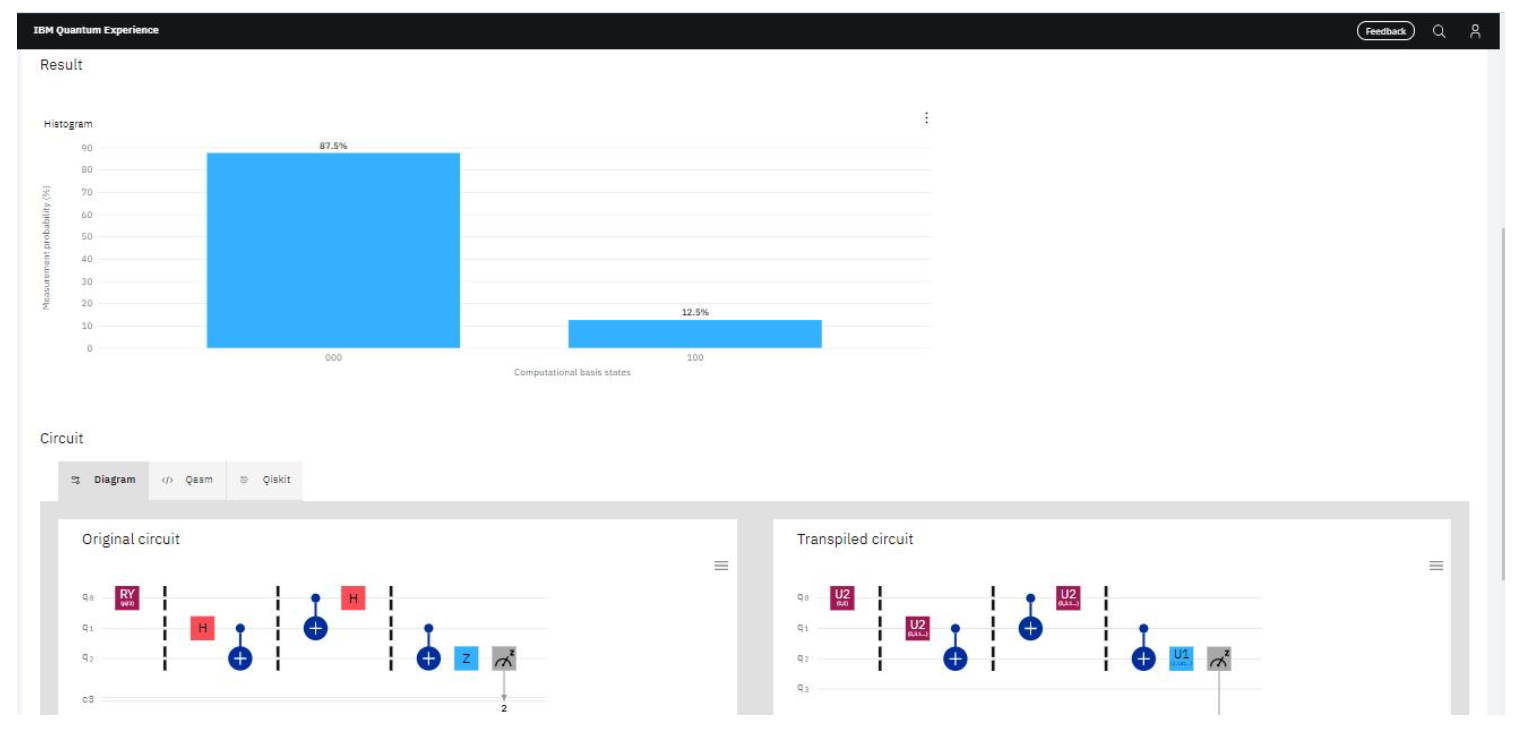
\includegraphics[scale=0.40]{5.2b/4.png}\\
            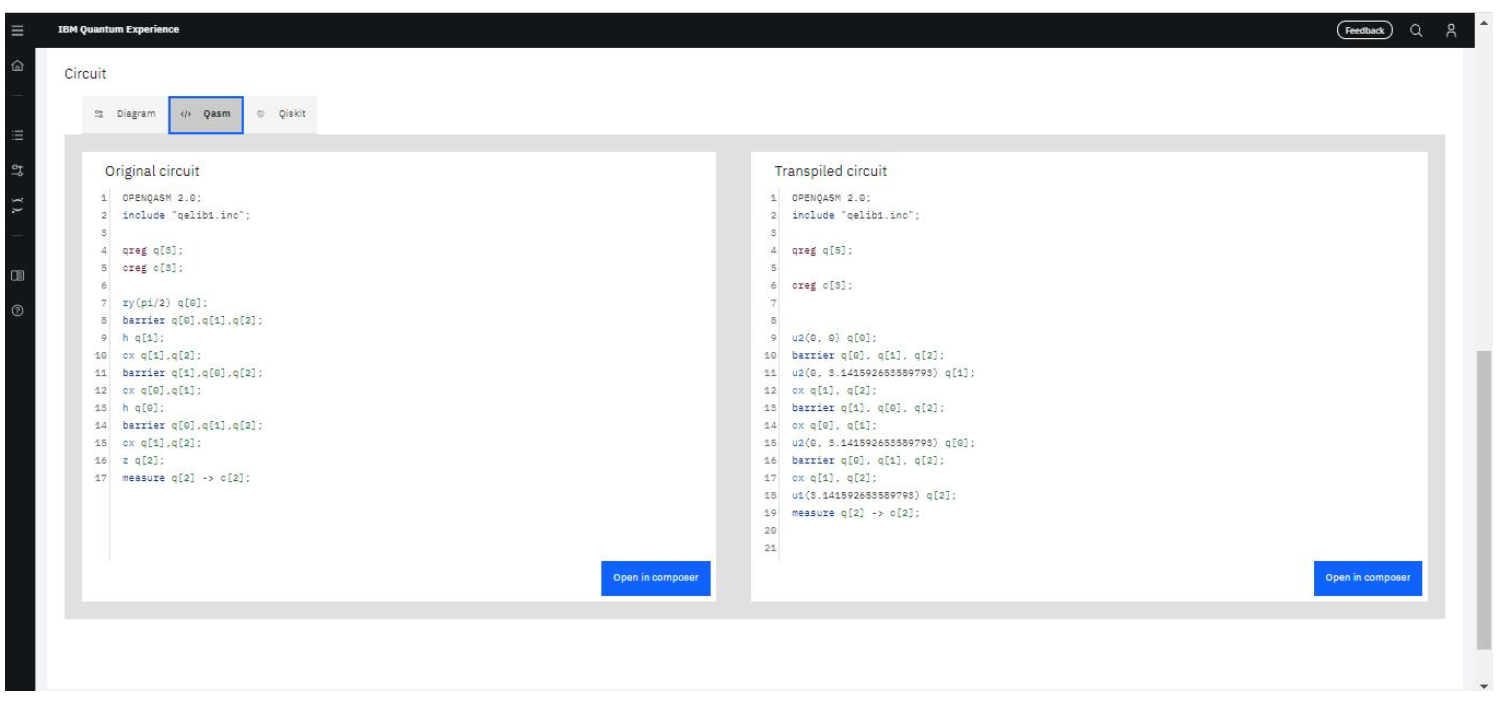
\includegraphics[scale=0.40]{5.2b/5.png}
    \item \phantom{-} \\
          \graphicspath{./5.2c/}
          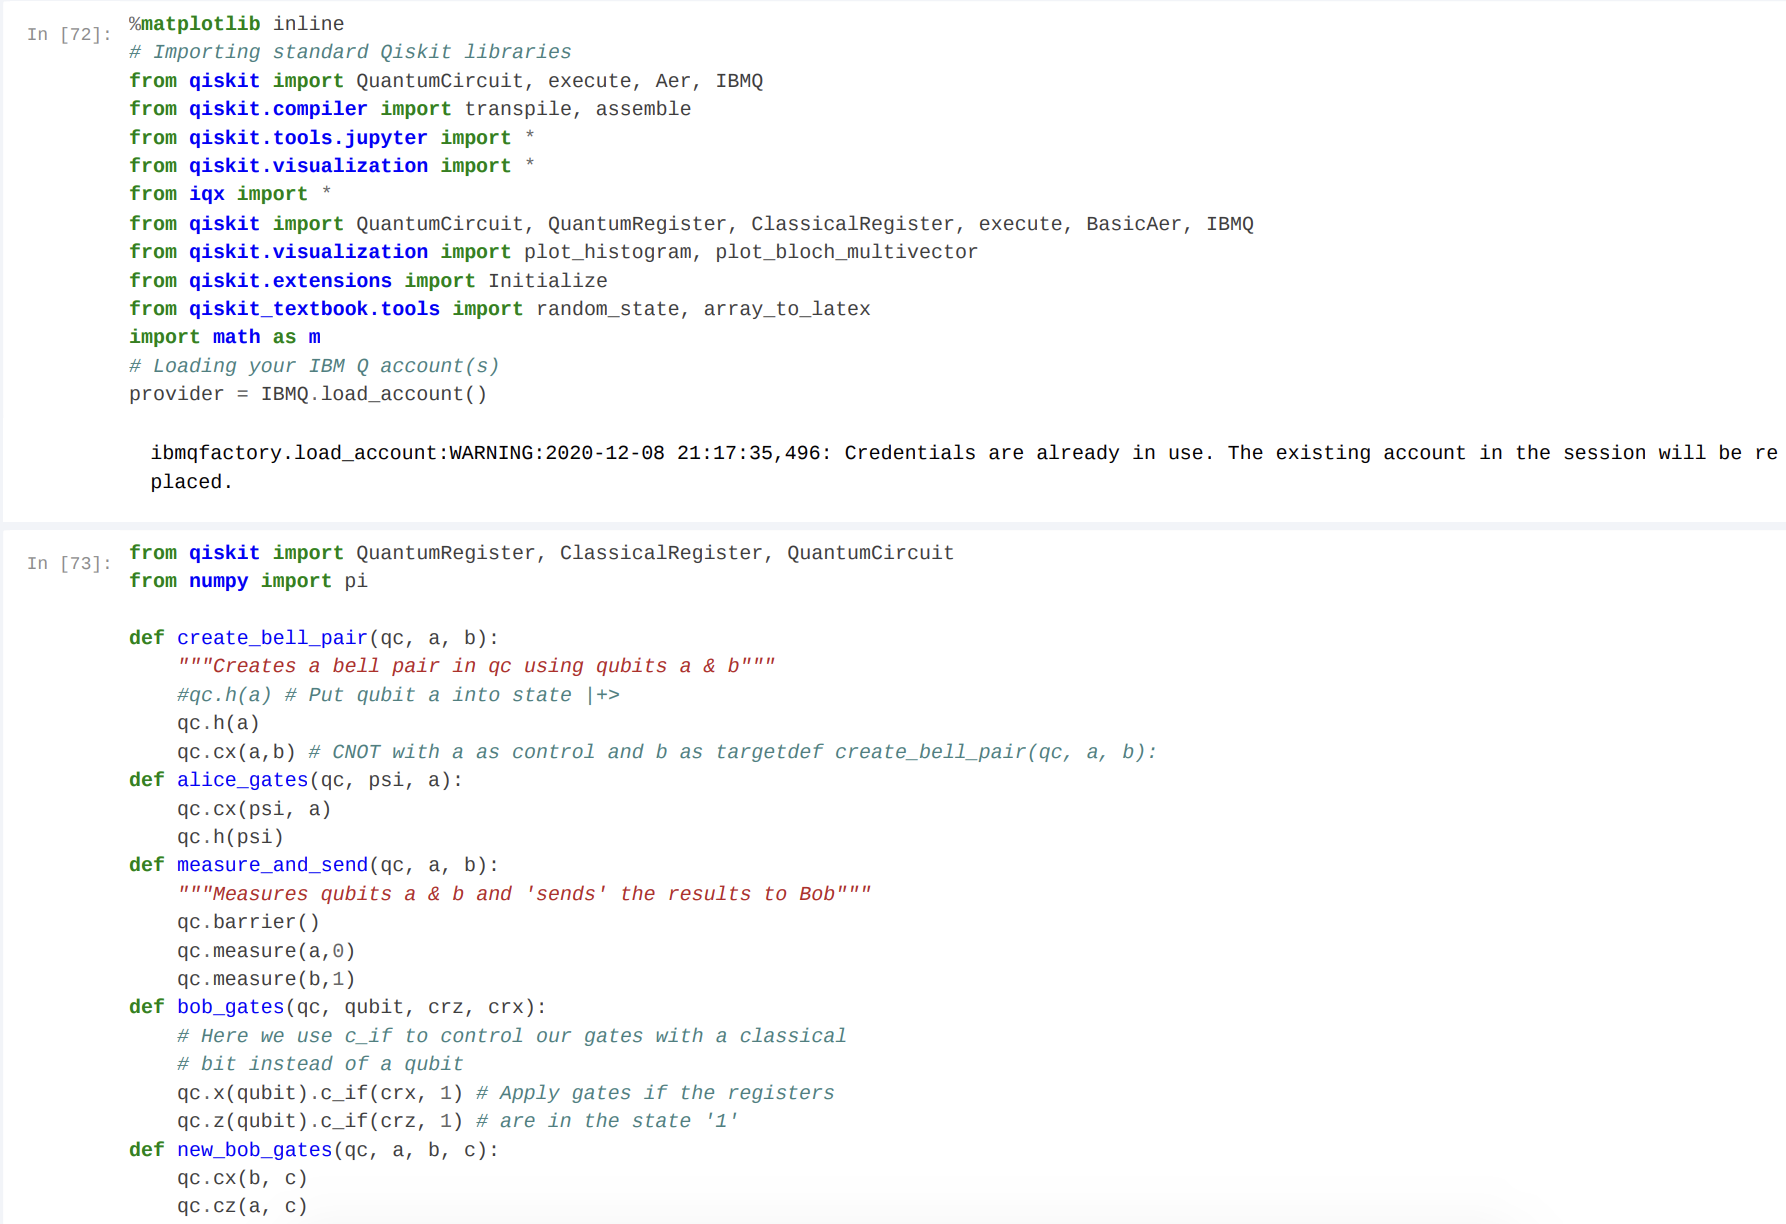
\includegraphics[scale=0.40]{5.2c/image1.png}\\
          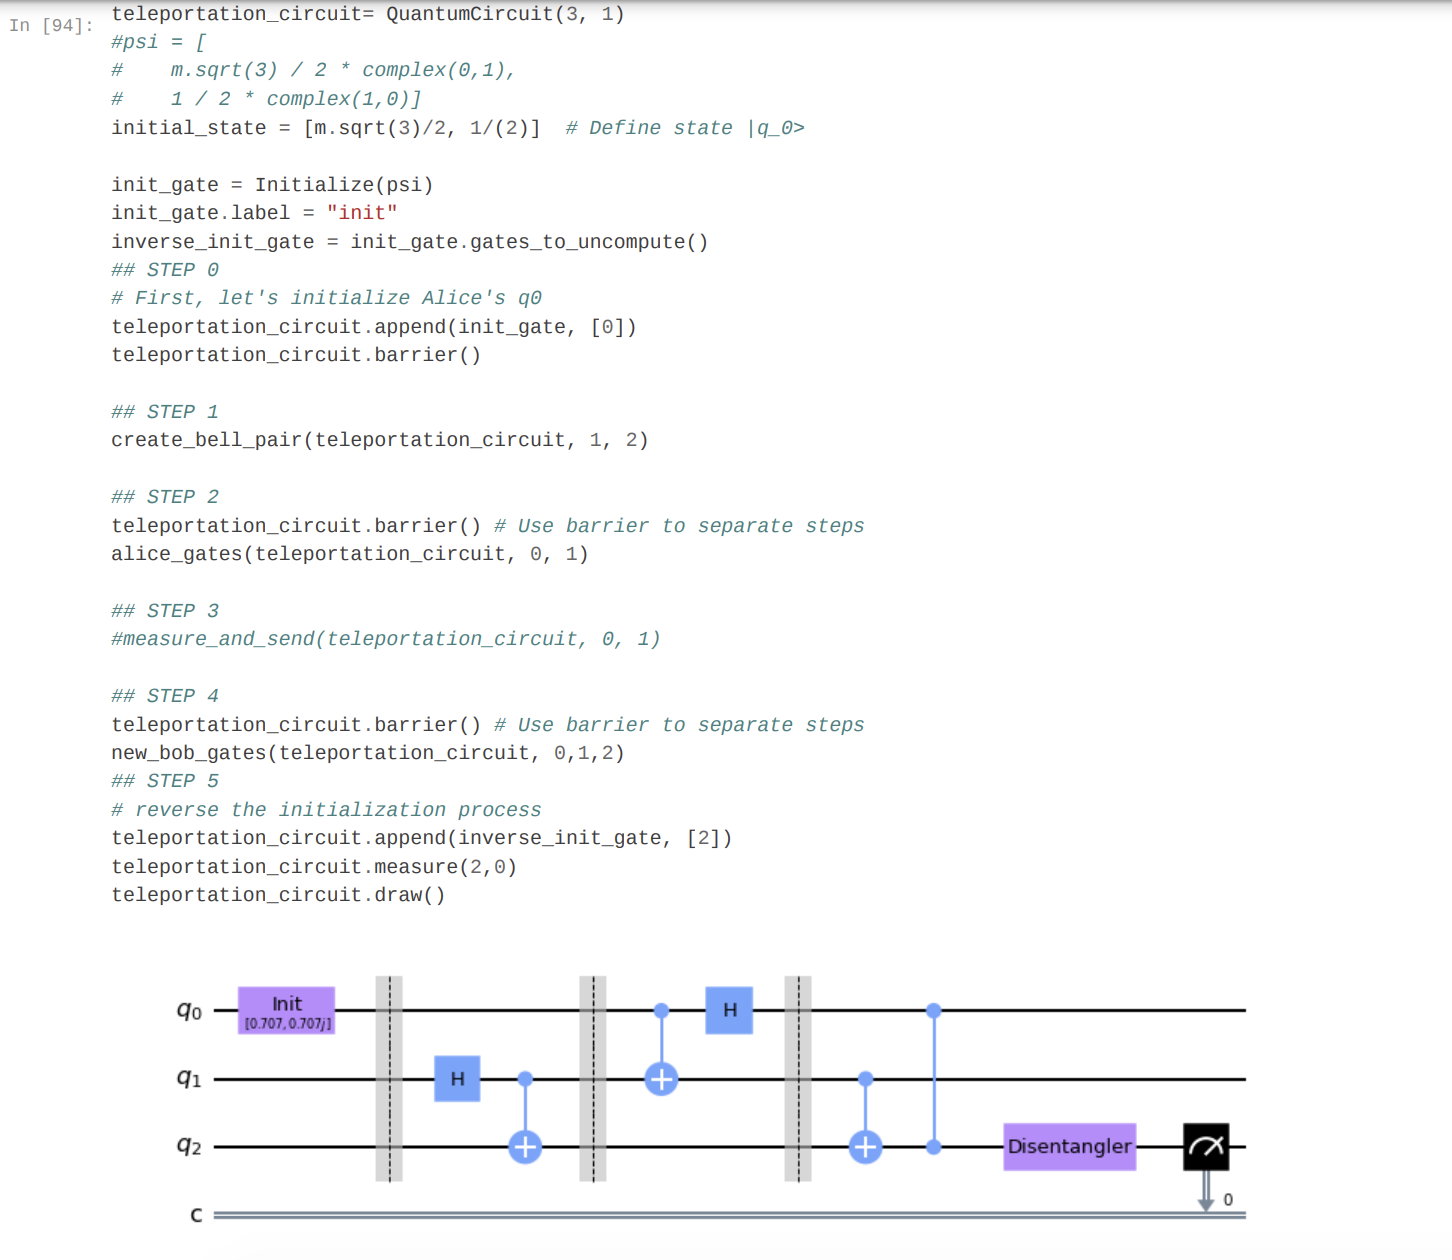
\includegraphics[scale=0.40]{5.2c/image2.png}\\
          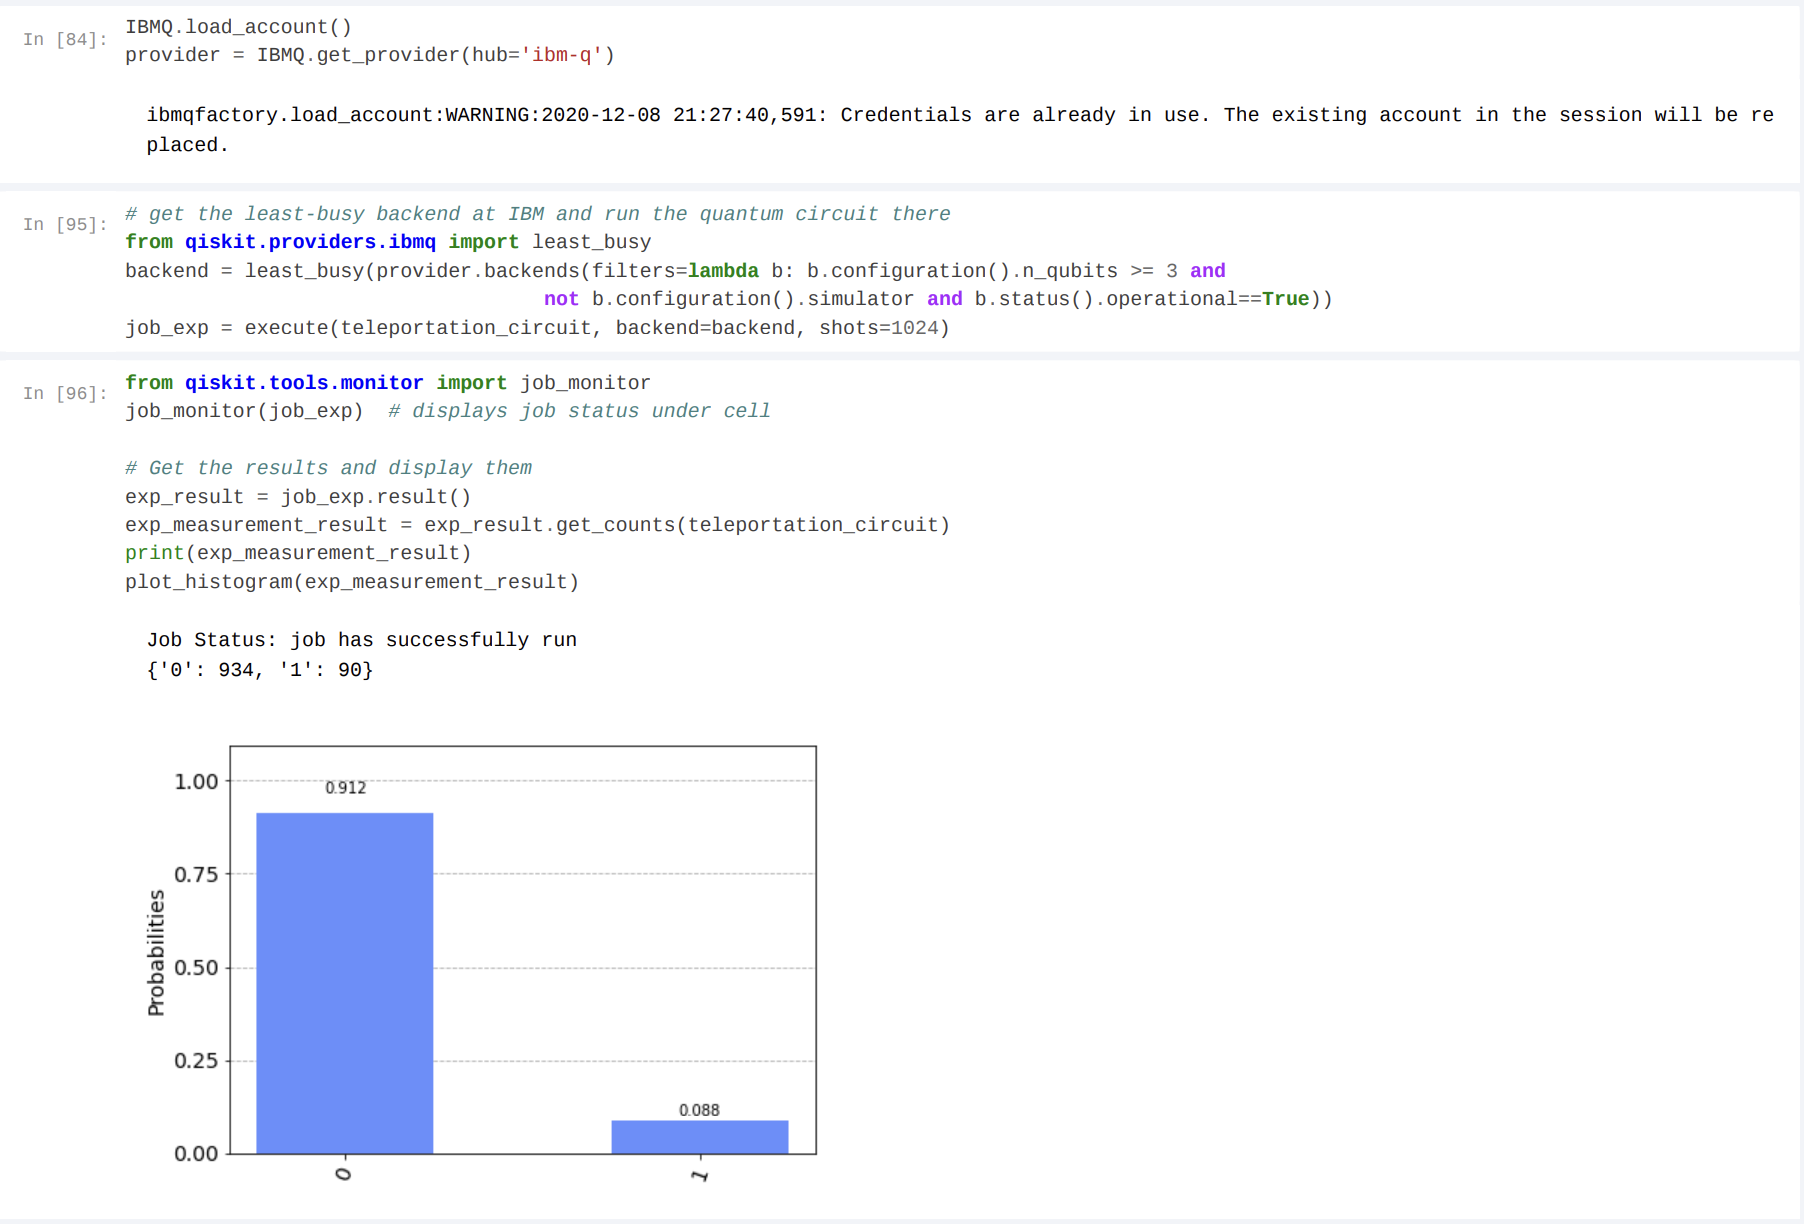
\includegraphics[scale=0.40]{5.2c/image3.png}\\
          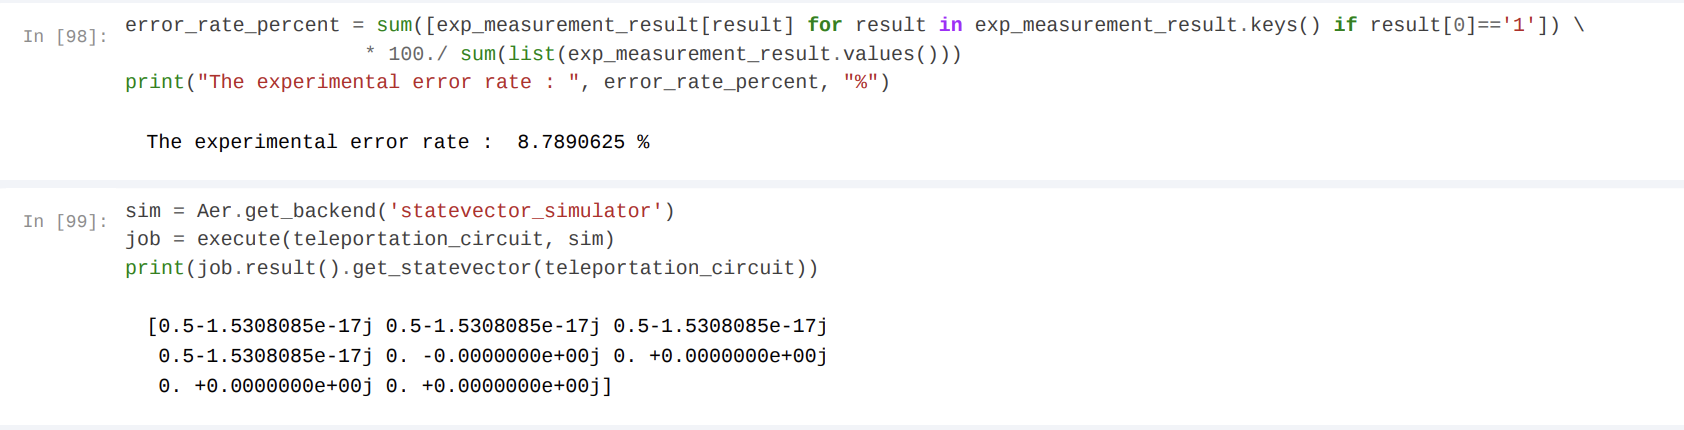
\includegraphics[scale=0.40]{5.2c/image4.png}
\end{enumerate}



\end{document}
